\documentclass{article}

\usepackage{xcolor}
\usepackage{listings}

\usepackage{minted}

\usepackage{xparse}
\usepackage{amsfonts}
\usepackage{amssymb}
\usepackage{mathtools}
\usepackage{braket}
\usepackage{forloop}
\usepackage{amsthm}
\usepackage{csquotes}
\usepackage{pdfpages}
\usepackage[pdftex,pdfpagelabels,bookmarks,hyperindex,hyperfigures,hidelinks]{hyperref}
\usepackage[backend=biber]{biblatex}
\usepackage{etoolbox}
\usepackage{nameref}
\usepackage[a4paper, total={6in, 8in}]{geometry}
\usepackage{authblk}
\usepackage{titlepic}
\usepackage{ulem}
\makeatletter
\def\uwave{\bgroup \markoverwith{\lower3.5\p@\hbox{\sixly \textcolor{red}{\char58}}}\ULon}
\font\sixly=lasy6 % does not re-load if already loaded, so no memory problem.
\makeatother

\AtBeginEnvironment{quote}{\par\singlespacing\small}

\newcommand{\spellerr}[2]{{\uwave{#1}\footnote{#2}}}
\newcommand{\cpp}[1]{{\mintinline{cpp}{#1}}}
\newcommand*{\fullref}[1]{\hyperref[{#1}]{\nameref*{#1} (\ref*{#1})}}

\lstset{language=C++,keywordstyle={\bfseries \color{CornflowerBlue}}}
\usemintedstyle{vs}


% huge align
\newcommand{\ha}[1]{{\huge{\begin{align*}#1\end{align*}}}}



% P & S Are excluded 
% \newcommand{\A}[0]{{\mathbb A}}
% \newcommand{\B}[0]{{\mathbb B}}
% \newcommand{\C}[0]{{\mathbb C}}
% \newcommand{\D}[0]{{\mathbb D}} 
% \newcommand{\E}[0]{{\mathbb E}} 
% \newcommand{\F}[0]{{\mathbb F}} 
% \newcommand{\G}[0]{{\mathbb G}} 
% \newcommand{\H}[0]{{\mathbb H}} 
% \newcommand{\I}[0]{{\mathbb I}} 
% \newcommand{\J}[0]{{\mathbb J}} 
% \newcommand{\K}[0]{{\mathbb K}} 
% \newcommand{\L}[0]{{\mathbb L}} 
% \newcommand{\M}[0]{{\mathbb M}} 
\newcommand{\N}[0]{{\mathbb N}}
% \newcommand{\O}[0]{{\mathbb O}} 
% \newcommand{\P}[0]{{\mathbb P}} 
\newcommand{\Q}[0]{{\mathbb Q}}
\newcommand{\R}[0]{{\mathbb R}}
% \renewcommand{\S}[0]{{\mathbb S}}
% \newcommand{\T}[0]{{\mathbb T}}
% \newcommand{\U}[0]{{\mathbb U}}
% \newcommand{\V}[0]{{\mathbb V}}
% \newcommand{\W}[0]{{\mathbb W}}
% \newcommand{\X}[0]{{\mathbb X}}
% \newcommand{\Y}[0]{{\mathbb Y}}
\newcommand{\Z}[0]{{\mathbb Z}}

% Calculus
% \newcommand{\d}[0]{{\mathrm{d}}}
\newcommand{\deriv}[2]{ \frac{ \d{#1} }{ \d{#2} } }
\newcommand{\pderiv}[2]{ \frac{ \partial{#1} }{ \partial{#2} } }

\newcommand{\nderiv}[3]{ \frac{ \d^{#1}{#2} }{ \d{#3}^{#1} } }
\newcommand{\npderiv}[3]{ \frac{ \partial^{#1}{#2} }{ \partial{#3}^{#1} } }

% Linear Algebra 
\renewcommand{\vector}[1]{ \overrightarrow{#1} }
\newcommand{\vecn}[1]{ {\hat #1} }

\newcommand{\mat}[1]{{ \begin{bmatrix} #1 \end{bmatrix} }}
\newcommand{\mats}[1]{{ \ba{\begin{smallmatrix} #1 \end{smallmatrix}} }}

\newcommand{\pmat}[1]{{ \begin{pmatrix} #1 \end{pmatrix} }}
\newcommand{\pmats}[1]{{ \pa{\begin{smallmatrix} #1 \end{smallmatrix}} }}

\newcommand{\emat}[1]{{ \begin{ematrix} #1 \end{ematrix} }}
\newcommand{\emats}[1]{{ \begin{smallmatrix} #1 \end{smallmatrix} }}

\newcommand{\vmat}[1]{{ \begin{vmatrix} #1 \end{vmatrix} }}

\newcommand{\rowechelon}[1]{{
			\left[\begin{array}{ccc|c} #1 \end{array}\right]
		}}

\newcommand{\augmented}[2]{{
			\left[\begin{array}{#1} #2 \end{array}\right]
		}}

% Generic Notatino
\newcommand{\paren}[1]{{ \left(#1\right) }}

\newcommand{\pa}[1]{{ \left(#1\right) }}
\newcommand{\ba}[1]{{ \left[#1\right] }}


\newcommand{\llet}[0]{ {\text{let } } }
\newcommand{\undefined}[0]{ {\text{undefined.} } }

\newcommand{\op}[1]{ {\operatorname{#1} } }

\newcommand{\brt}[2]{ {\root {#1} \of {#2} } }

\newcommand{\proj}[1]{ { \op{proj}_{#1} }}
\newcommand{\projperp}[1]{ { \op{proj}_{#1\perp} } }

\newcommand{\norm}[1]{{ {\left\lVert #1 \right\rVert} }}
\newcommand{\norms}[1]{{ {\lVert #1 \rVert} }}

% CS 
\newcommand{\hex}[1]{{ \pa{\mathrm{#1}}_{16} }}
\newcommand{\bin}[1]{{ \pa{#1}_{2} }}
\newcommand{\binb}[2]{{ \pa{#1}^{#2}_{2} }}
\newcommand{\dec}[1]{{ \pa{#1}_{10} }}


\newcommand{\true}[0]{{ \mathrm{true} }}
\newcommand{\false}[0]{{ \mathrm{false} }}

\renewcommand{\ba}[1]{{ \left[ {#1} \right] }}

\newcommand{\ceil}[1]{{ \left\lceil {#1} \right\rceil }}
\newcommand{\floor}[1]{{ \left\lfloor {#1} \right\rfloor }}

\newcommand{\ang}[1]{{ \left\langle {#1} \right\rangle }}

\newcommand{\transpose}[1]{ { {#1}^{\intercal} } }





\addbibresource{references.bib}

\title{CS280 Assignment - Lariat}
\date{ }
\author[1]{Luke Cardell}
\author[2]{Slightly modified by Dmitri Volper}
\author[3]{Translated to PDF by Kishan S Patel}
\affil[1]{Digipen Institute of Technology}

\newcommand{\volpy}[1]{{
\includegraphics[width=#1\textwidth]{myman.png}}}
\newcommand{\surprisevolpy}[0]{{\volpy{0.02}}}

\titlepic{\volpy{0.3}}

\begin{document}

\maketitle


\pagebreak
\tableofcontents
\pagebreak


\begin{section}{What is Lariat}

 \begin{displayquote}
	 It is important to understand that this is not the only way to solve this
	 assignment, merely the way that worked best for me.
 \end{displayquote}

 \indent Under the hood, Lariat looks like a "linked list of arrays".

 \indent The main goal is to have a more efficient (compared to array) insert in the
 middle.
 Reminder: if array (and consequently \mintinline{cpp}{std::vector}) insert an element
 in the middle, all elements to the right of the insert position have to be
 shifted 1 position to the right to free a spot for new element. This is $O(N)$ (linear) operation. Another possible problem is if there is not \uwave{anough}\footnote{enough} space,
 which will required reallocation if the whole array.
 Lariat solves the problem by storing small segments of contiguous memory non-contiguously.


 During insert one of $2$ things can happen (see \uwave{datail}\footnote{detail} later):
 \begin{itemize}
	 \item the contiguous block may have extra space, so only some elements have to be shifted
	       \begin{minted}[autogobble]{cpp}
//    0  1            2  3  4        // index
// +------------+  +------------+
// |  1  3     -|->|  4  5  6  -|->  // data
// +------------+  +------------+
// after insert 2 before 3
//    0  1  2         3  4  5         6  7  8
// +------------+  +------------+  +------------+
// |  1  2  3  -|->|  4  5  6  -|->|  9  9  9  -|->
// +------------+  +------------+  +------------+
// only value 3 had to shifted
	\end{minted}

	 \item block containing insert position is full, then we split it
	       \begin{minted}[autogobble]{cpp}
// insert 8 before 5
// first split:
//    0  1  2         3  4            5  6            6  7  8       
// +------------+  +------------+  +------------+  +------------+  
// |  1  2  3  -|->|  4  8     -|->|  5  6     -|->|  9  9  9  -|->
// +------------+  +------------+  +------------+  +------------+  
// now insert
//    0  1  2         3  4            5  6            7  8  9       
// +------------+  +------------+  +------------+  +------------+    
// |  1  2  3  -|->|  4  8     -|->|  5  6     -|->|  9  9  9  -|->
// +------------+  +------------+  +------------+  +------------+    
// only values 5 and 6 were copied
			\end{minted}
 \end{itemize}


\end{section}

\begin{section}{Luke's Guide to Templated Templates}

 \begin{displayquote}
	 "We put some templates in your templates so you could generate code at compile
	 time while you generate code at compile time."
	 -C++
 \end{displayquote}

 \indent A template is a section of code like any other that gets "written" at compile
 time, rather than when you actually write templated code. In this sense,
 writing a template is about using the compiler to your own advantage to avoid
 doing unnecessary work.

 \begin{displayquote}
	 Laziness FTW\footnote{For the Win}
 \end{displayquote}


 A normal function template is \spellerr{declard}{declared} as such:
 \begin{minted}[autogobble]{cpp}
		template<typename T>
		void Foo(T bar);
	\end{minted}

 The definition requires knowledge of the template parameters in order to work:

 \begin{minted}[autogobble]{cpp}
		template<typename T>
		void Foo<T>(T bar) {
			//     |
			//      `-[function template ]

			//...
		}
	\end{minted}

 \indent In the Lariat assignment, you will have to make a templated copy constructor
 and assignment operator for the Lariat template class. This is similar to
 writing a static function template, but it's written within another
 encompassing template, the Lariat class in this case.

 \indent The basic declaration of the function is just like a normal template
 function, but within a class scope.

 \begin{minted}[autogobble]{cpp}
		template<typename T>
		class Foo {
			//...

			template<typename Bar>
			void Baz(Bar & qux);

			//...
		};
	\end{minted}

 \pagebreak
 \indent The definition of the function takes a little bit more work, which may be confusing at first.


 \begin{minted}[autogobble]{cpp}
    template<typename T>    // Gives the external class template information
    template<typename Bar>  // Gives the internal function template information
		void Foo<T>::Baz<Bar>(Bar & qux) {
      // |          |
      // |           `-[function signature]
      //  `-[class namespace]

      // ...
    }
 \end{minted}


 \indent The first template declaration belongs to the class, which may be instantiated
 multiple times with multiple name-mangled signatures based on the compiler's
 implementation of templates.

 \indent The second template declaration belongs to the function, which will likely be
 instantiated multiple times for every single class instantiation. In this way
 the structure resembles a tree:


 \begin{figure}[h]
	 \centering
	 \begin{verbatim}
										+-source------------------------------+
										| original code written by programmer |
										+-------------------------------------+
											 /                               \
					 +-class---------+                     +-class---------+
					 | instantiation |                     | instantiation |
					 | for type A    |                     | for type B    |
					 +---------------+                     +---------------+
					 /               \                     /               \
+-function------+ +-function------+      +-function------+ +-function------+
| type A        | | type B        |      | type A        | | type B        |
| instantiation | | instantiation |      | instantiation | | instantiation |
+---------------+ +---------------+      +---------------+ +---------------+
	\end{verbatim}
	 \caption{\#dat\_ascii\surprisevolpy}
 \end{figure}



 \pagebreak
 \indent The next little template trick you might run into with this assignment comes
 when you try to refer to internal member types in the instantiation of code.
 I personally used this in my helper functions that returned pointers to nodes
 in the list, but it's useful for any further template work you might be
 interested in doing.

 \indent Dependent types are also instantiated for \spellerr{ech}{each} class, with the exact same
 process as function templates. This means that using just the internal name
 in external code will lead to type confusion, where the compiler isn't sure
 which owning class is being referred to.

 \indent A class class template with a member type and a member function returning a
 pointer to the member type:

 \begin{minted}[autogobble]{cpp}
    template<typename T>
    class Foo {
      //...

      struct Bar {
        //...
      }

      Bar * Baz();

      //...
    };
 \end{minted}

 The member function here must be defined as such:
 \begin{minted}[autogobble]{cpp}

    template<typename T>
		typename Foo<T>::Bar * Foo<T>::Baz() {
      // |       |    |       |     |
      // |       |    |       |      `-[function signature]
      // |       |    |        `-[class namespace]
      // |       |     `-[member typename]
      // |        `-[class namespace]
      //  `-[declaration of token as user-defined type]

      //...
    }
 \end{minted}

 \pagebreak
 \indent The last real trick I want to share with you pertains directly to the copy
 constructors this assignment requires. At their instantiation, class templates
 only have direct access to their own \spellerr{instatiation's}{instantiation's} member variable. This
 means that in order to see another instantiation's private variables, there
 must be a declaration of each instantiation as a friend.

 \begin{displayquote}
	 How do you make something to account for any scenario at compile time?

	 Simple. More templates.

	 Declare a friend class template in your original class template.

	 \begin{minted}[autogobble]{cpp}
    template<typename T>>
    class Foo {
      //...

      template<typename U>  //[nested template declaration]
      friend class Foo<U>;  //[friend declaration for class template]

      //...
    }
	 \end{minted}
 \end{displayquote}

 \indent This has been my brief introduction to templates as they pertain to this
 assignment. they may seem scary, but templates allow for a greater depth and
 elegance of code, decreasing the total writing time and reducing the volume of
 duplicated code.

\end{section}

\section{Assignment Details}

\subsection{Lariat Class Details}


\subsubsection{Template Parameters}
\indent The \cpp{Lariat} class has two template parameters which are generally self-
explanatory.
\\

\begin{tabular}{|c|c|}
	\hline
	\mintinline{cpp}{typename T} & The type of data being stored in the data structure \\
	\hline
	\mintinline{cpp}{int Size}   & The logical size of the arrays within the node      \\
	\hline
\end{tabular}



\subsubsection{Member Variables}
\indent The \cpp{Lariat} class provided by Volper\footnote{\surprisevolpy} has five member variables.
\\


\begin{tabular}{|c|c|}
	\hline
	\mintinline{cpp}{head_}      & A pointer to the first node in the linked list                       \\
	\hline
	\mintinline{cpp}{tail_}      & A pointer to the last node in the linked list                        \\
	\hline
	\mintinline{cpp}{size_}      & An integer for the total number of elements actively storing data    \\
	\hline
	\mintinline{cpp}{nodecount_} & An integer for the number of nodes in the linked list                \\
	\hline
	\mintinline{cpp}{asize_}     & An integer for the size of the array within each node                \\
	                             & Interchangeable with the template parameter \mintinline{cpp}{<Size>} \\
	\hline
\end{tabular}


\subsubsection{Member Type}

\indent The \cpp{Lariat} class has one member type, the \cpp{LNode} struct used in the linked
list internal implementation. \cpp{LNode} has four member variables of its own.
\\

\begin{tabular}{|c|c|}
	\hline
	\cpp{next}   & A pointer to the next node in the linked list                                \\
	\hline
	\cpp{prev}   & A pointer to the previous node in the linked list                            \\
	\hline
	\cpp{count}  & An integer to track of how many elements the \cpp{LNode} is actively storing \\
	\hline
	\cpp{values} & An array of \cpp{<Size>} elements of type \cpp{<T>}                          \\
	\hline
\end{tabular}





\pagebreak
\subsection{Function Details}


\indent Remember to check for null at any point you're dealing with pointers. In
particular, make sure to check if the head and tail are null before you try
to work with them. I find that not dereferencing null is generally the better
programming practice.

\indent Also remember to update the \cpp{size_} and \cpp{nodecount_} member variables where
necessary.


\begin{itemize}
	\item Constructors and Destructor
	      \begin{itemize}
		      \item[-] ctor
		      \item[-] copy ctor (own-type)
		      \item[-] copy ctor (template)
		      \item[-] dtor
	      \end{itemize}
	\item Assignment Operators
	      \begin{itemize}
		      \item[-] \cpp{operator=} (own-type)
		      \item[-] \cpp{operator=} (template)
	      \end{itemize}
	\item Element Addition
	      \begin{itemize}
		      \item[-] \cpp{insert}
		      \item[-] \cpp{push_back}
		      \item[-] \cpp{push_front}
	      \end{itemize}
	\item Element Removal
	      \begin{itemize}
		      \item[-] \cpp{erase}
		      \item[-] \cpp{pop_back}
		      \item[-] \cpp{pop_front}
	      \end{itemize}
	\item Element Access
	      \begin{itemize}
		      \item[-] \cpp{operator[]}
		      \item[-] \cpp{first}
		      \item[-] \cpp{last}
	      \end{itemize}
	\item Data Structure Information
	      \begin{itemize}
		      \item[-] \cpp{find}
		      \item[-] \cpp{size}
	      \end{itemize}
	\item Data Structure Control
	      \begin{itemize}
		      \item[-] \cpp{clear}
		      \item[-] \cpp{compact}
	      \end{itemize}
	\item Recommended Helper Functions
	      \begin{itemize}
		      \item[-] \cpp{split}
		      \item[-] \cpp{findElement}
		      \item[-] \cpp{shiftUp}
		      \item[-] \cpp{shiftDown}
	      \end{itemize}
\end{itemize}


\pagebreak
\subsection{Constructors and Destructor}


\subsubsection{Constructor}
\indent This constructor is really simple. You don't need to do any logic, just
use a member initializer list to initialize

\subsubsection{Copy Constructor (own-type)}
\indent This is the standard copy constructor. The function should loop through the
instance passed in, pushing each element of the other onto the back of
the one being constructed.

\indent It should be done using the algorithm for (or directly calling) \cpp{push_back}
so that all of the nodes are split correctly.

\subsubsection{Copy Constructor (template)}
\indent This copy constructor is algorithmically identical to the own-type
constructor, but is templated to allow for a Lariat type instantiation
with different parameters for \cpp{<T>} and \cpp{<Size>}.

\indent Refer to the above guide to templates for details on how to write the
function signature.

\subsubsection{Destructor}
The destructor is a simple, generic destructor. It's sole purpose is to
free all the nodes in the linked list so there are no memory leaks.


\pagebreak
\subsection{Assignment Operators}

\subsubsection{\cpp{operator=} (own-type)}
\indent This assignment operator generally works exactly the same as you might
expect. Set the non-pointer members as necessary, clear this instance's
data, then walk through the right-hand argument's list adding each
element to this instance

\subsubsection{\cpp{operator=} (template)}
\indent This assignment operator follows the exact same algorithm as the own-type
version, but is a nested template like I described above.


\pagebreak
\subsection{Element Addition}


\subsubsection{\cpp{insert}}
\label{func:insert}

\indent Insert an element into the data structure at the index, between the element
at \cpp{[index - 1]} and the element at \cpp{[index]}
The first thing to this function is to check for an Out of Bounds error. If
the index is invalid, throw a \cpp{LariatException} with \cpp{E_BAD_INDEX} and the
description "Subscript is out of range"
Make sure to handle the "edge\footnote{
\includegraphics[width=0.025\textwidth]{edge.jpg}}" cases, which allow for insertion at the end
of the deque as well as the beginning. I personally suggest calling
\cpp{push_back} and \cpp{push_front} in these cases, as it helps minimize the amount
of code written and the algorithm is identical anyways.

\indent The next thing to do is to set up the actual insertion algorithm.
First, find the node and local index of the element being inserted. This
can be done with the \cpp{findElement} helper function detailed in the
Recommended Helper Functions section of this guide.

Next, shift all elements past that local index one element to the right.
This can be done with the \cpp{shiftUp} function detailed in \fullref{section:rec_helper}.

\begin{minted}[autogobble]{cpp}
      /*
            [e]
             |
             v
        +------------------+      (0) Starting position, inserting 'e' at
        |[a][b][c][d][_][_]|          index 1 of the node
        +-0--1--2--3--4--5-+

            [e]
             |
             v
        +------------------+      (1) Shift all elements right from index
        |[a][_][b][c][d][_]|
        +-0--1--2--3--4--5-+

            [_]
             |
             v
        +------------------+      (2) Set the newly open element to the value
        |[a][e][b][c][d][_]|          being inserted, 'e' here
        +-0--1--2--3--4--5-+
      */
\end{minted}


\pagebreak

\indent This should work for the most common use-case, but it will cause a
problem if the node is full.
If the node is full, you will need to keep track of the last element in
the node before you shift all the elements to the right. Again, this is
easy to do with the recommended helper function.
I call this "popped off" element the overflow.

\begin{minted}[autogobble]{cpp}
      /*
            [g]
             |            [_]
             v            /
        +------------------+      (0) Starting position, inserting 'g' at
        |[a][b][c][d][e][f]|          index 1 of a full node
        +-0--1--2--3--4--5-+

            [g]
             |            [f] <-[overflow]
             v            /
        +------------------+      (1) Shift all elements right from index,
        |[a][_][b][c][d][e]|          keeping track of the overflow, 'f' here
        +-0--1--2--3--4--5-+

            [_]
             |            [f]
             v            /
        +------------------+      (2) Set the newly open element to the value
        |[a][g][b][c][d][e]|          being inserted, 'g' here
        +-0--1--2--3--4--5-+
      */
\end{minted}

\indent Next, you will need to split the node.
I would recommend writing a helper function for this algorithm as it
will be used elsewhere. I have detailed the split algorithm in \fullref{section:rec_helper}.
You will need to transfer the overflow to the last element of the new
node created by the split. It is possible to put this part of the
algorithm directly in the split function. I will not detail that in
this guide, but rather leave it for you to discover on your own.
Working out that algorithm will probably make your code much cleaner,
so I would definitely recommend figuring it out.
As the split algorithm accurately updates the node counts for the split
nodes, the only thing left to do is increment the node count.




\subsubsection{\cpp{push_back}}
\indent This is an easy algorithm using the \cpp{split}  function (\ref{section:rec_helper}).

\begin{itemize}
	\item If the tail node is full, split the node and update the \cpp{tail_} pointer.
	\item Set the last element in the tail's array to the value.
	\item Increment the tail node's count.
\end{itemize}

\pagebreak
\subsubsection{\cpp{push_front}}
This algorithm is more similar to the \cpp{insert} function (\ref{func:insert}) than the \cpp{push_back}
algorithm, but is still relatively simple.

\begin{itemize}
	\item If the head node is empty, increment the node's count.
	\item If the head node is full, you will need to shift the elements up, in the
	      same way they were shifted in the insert function, making sure to track the overflow.
	\item Next you will need to split the node.
	      In order to account for splitting the only node in the linked list, you
	      will have to update the \cpp{tail_} pointer as necessary.
	\item If the head node isn't full yet, just shift the head node up an element
	      from element 0 and increase the count.
	\item Set the 0'th element of the head to the value.
\end{itemize}


\pagebreak
\subsection{Element Removal}


\subsubsection{\cpp{erase}}

This function uses the \cpp{findElement} helper function I have detailed in
\fullref{section:rec_helper}. Having implemented that, the function itself is relatively simple.
You can use the \cpp{pop_back} and \cpp{pop_front} functions if the index requested is
the first or last element.


\begin{itemize}
	\item First, find the containing node and local index of the requested global
	      index.
	\item Shift all the elements in the node beyond the local index left one element,
	      covering the element being erased. This is done with the \cpp{shiftDown}
	      function detailed in \fullref{section:rec_helper}. Make sure
	      to account for the node being only one element large.
	\item Decrement the node's count.
\end{itemize}


\subsubsection{\cpp{pop_back}}
Decrement the count of the tail node.

\subsubsection{\cpp{pop_front}}
Shift all elements in the head node down one element.
Decrement the head's count.

If the head node is now empty, free the associated memory.


\pagebreak
\subsection{Element Access}

\indent As the const and non-const versions of these functions are algorithmically
and syntactically identical, I would recommend (may \spellerr{Shilling}{Schilling 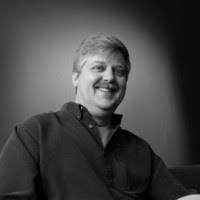
\includegraphics[width=0.02\textwidth]{schilldawg.jpg}} forgive me)
copy\/pasting the code from one to the other. You can't call one from inside
the other, as that would violate the const requirements.

\subsubsection{\cpp{operator[]}}
Find the containing node and local index of the index passed in. Like
insert and erase, this is easily done with the \cpp{findElement} helper
function I detailed in \fullref{section:rec_helper}.

Return the element at the local index of the containing node.

\subsubsection{\cpp{first}}
This is one of the easiest functions in this assignment.

Return the first element of the head node.

\subsubsection{\cpp{last}}
This is also an easy function.

Return the last element in the tail node.


\pagebreak
\subsection{Data Structure Information}

\subsubsection{\cpp{find}}
Walk the list in a similar fashion to that detailed in the \cpp{findElement}
helper function (\ref{section:rec_helper}), but check equivalence for each element in each node,
returning the index when the desired element is found.

If the desired element is not found, return the total number of elements
contained in the data structure.

\subsubsection{\cpp{size}}
You should be tracking the \cpp{size_} member variable throughout the element
addition and removal processes. Return that variable now.


\pagebreak
\subsection{Data Structure Control}

\subsubsection{\cpp{clear}}
\indent This is a relatively simple function with a similar algorithm to the
class destructor.

\begin{itemize}
	\item First, loop through the list, freeing each node in turn.
	\item Once the list is empty, update the necessary member variables.
\end{itemize}

\subsubsection{\cpp{compact}}
\indent Compact takes all the data stored in the linked list and moves it into the
smallest number of nodes possible. Then it frees all empty nodes at the
end of the list.

The algorithm for this walks the list at two points in parallel. I will
refer to the walker having elements shifted into it as the left foot and
the walker reading through the elements to shift as the right foot.

\begin{itemize}
	\item First, loop through the list with both feet until the left node is not
	      already full and the right foot hasn't walked off the list.
	\item Next, walk through the list while the right foot hasn't lost the list.

	\item This loop should first store the count of elements in the right node,
	      then set the count of the right node to zero. This allows the left foot
	      to update it as it is given elements to store.
	\item This loop should have a nested loop that stores each value from the right
	      foot in the left foot's node, and steps the left foot to the next node
	      when it is filled.
\end{itemize}


\begin{verbatim}
 ______________________________________  
|.-KEY--------------------------------.| 
|| [node]   [values]   [count]        || 
||   |         |           |  [next]  || 
||   v         v           v    |     || 
||  +-+-node-------------+---+  v     || 
||  |#|[_][_][_][_][_][_]|(_)| --->   || 
||  +-+------------------+---+        || 
||      0  1  2  3  4  5  <-[indices] || 
||____________________________________|| 
'--------------------------------------' 
\end{verbatim}


\begin{enumerate}

	\item The starting position of the inner loop, \spellerr{transfering}{transferring} right's first
	      element into left's fifth space

	      \begin{verbatim}
                                 [rpos = 0]                           
                                     |                      [rtot = 3]
 +-+-left-------------+---+      +-+-right------------+---+      +-+-...
 |0|[a][b][c][d][_][_]|(4)| ---> |1|[e][f][g][_][_][_]|(0)| ---> |2|[...
 +-+------------------+---+      +-+------------------+---+      +-+-...
     0  1  2  3  4  5                0  1  2  3  4  5                 					
			 \end{verbatim}


	\item Next important point, the left foot is now full. Set the left foot
	      to the next node in the list and continue the algorithm
	      \begin{verbatim}
                                       [rpos = 2]                     
                                           |                [rtot = 3]
 +-+-left-------------+---+      +-+-right------------+---+      +-+-...
 |0|[a][b][c][d][e][f]|(6)| ---> |1|[_][_][g][_][_][_]|(0)| ---> |2|[... 
 +-+------------------+---+      +-+------------------+---+      +-+-...				
     0  1  2  3  4  5                0  1  2  3  4  5                 				
			 \end{verbatim}


	\item Left and right feet are now standing on the same node, but the
	      algorithm still works because it is based on index in the node
	      rather than the node itself.
	      \begin{verbatim}
        [rpos = 2]                                                     
            |                                                [rtot = 3]
  +-+-left/right-------+---+      +-+-right->next------+---+      +-+-... 
  |1|[_][_][g][_][_][_]|(0)| ---> |2|[h][i][j][k][_][_]|(4)| ---> |3|[... 					
  +-+------------------+---+      +-+------------------+---+      +-+-...					
      0  1  2  3  4  5                0  1  2  3  4  5                 				
		\end{verbatim}


	\item The left foot has had the element at rpos shifted down, and the
	      right foot has stepped to the next node. Note that rtot has been
	      updated to 4, the right node has had its count zeroed out, and
	      rtot has been updated to the right node's original count.


	      \begin{verbatim}
                                    [rpos = 1]                        				
                                        |                   [rtot = 4]
 +-+-left-------------+---+      +-+-right------------+---+      +-+-... 
 |1|[g][h][_][_][_][_]|(2)| ---> |2|[_][i][j][k][_][_]|(0)| ---> |3|[...
 +-+------------------+---+      +-+------------------+---+      +-+-...
     0  1  2  3  4  5                0  1  2  3  4  5                 
				\end{verbatim}


\end{enumerate}

Once the deque has been compacted, remove all the extra nodes from the
end of the list.


\pagebreak
\section{Recommended Helper Functions}
\label{section:rec_helper}


\subsubsection{\cpp{clear}}
This is a relatively simple function with a similar algorithm to the
class destructor.

\begin{itemize}
	\item First, loop through the list, freeing each node in turn.
	\item Once the list is empty, update the necessary member variables.
\end{itemize}




\end{document}
